%Tipo de pesquisa e sua justificativa
Este trabalho se trata de um estudo de caso, pois se avalia o \textit{Lean Learning} em um contexto da vida real, com finalidade de pesquisa empírica, visando aprofundar os estudos na área \cite{MIGUEL2007}. Além disso, não há aprioristicamente um esquema estrutural, não tendo um problema e variáveis já definidas previamente, portanto seu objetivo é apreender determinada situação e descrever o caso observado\cite{marconi2003fundamentos}\cite{marconi2012tecnicas}. Também é descritivo, já que apresenta uma descrição exaustiva de um fenômeno, dentro do respectivo contexto \cite{Eduser} a fim de refinar os estudos sobre a teoria \cite{MIGUEL2007}. Envolve medidas qualitativas como a satisfação dos alunos e do professor com as atividades propostas com o \textit{Lean Learning} e gera métricas quantitativas para análise geral dos resultados obtidos, como a média da satisfação geral dos alunos quanto às atividades realizadas \cite{Metricas}. Como objeto de estudo do trabalho tem-se a etapa \textit{Measure} (Medir) do \textit{Lean Learning}.

Com os dados coletados, é conduzida a fase de análise dos mesmos. Procura-se observar possíveis padrões presentes nas métricas abordadas no trabalho, e descrever situações que foram benéficas para a satisfação dos alunos. A cada questionário fechado analisado, é definida a média das métricas coletadas em relação a todos os alunos respondentes. Além disso, através de um \textit{script} R, será possível estabelecer quais perguntas possuem correlação com as métricas estudadas, através do uso da função \textit{cfa()} (de Análise Fatorial Confirmatória), da biblioteca lavaan (\textit{latent variable analysis}). 

As nove perguntas relativas às práticas presentes no questionário fechado dos alunos foram agrupadas em três tipos: três perguntas para medir satisfação (S), três perguntas para medir adequação (A) e três perguntas para medir a proximidade da prática com o mercado (M). O primeiro grupo visa avaliar a satisfação dos alunos com a realização da prática. O segundo visa avaliar a opinião dos alunos sobre sua adequação à prática, em termos de cumprimento, dificuldade e tempo disponível. O terceiro e último visa avaliar a opinião dos alunos sobre o quanto a prática reflete a realidade do mercado de trabalho de \textit{software}.

A fórmula para a especificação de modelos de regressão no Lavaan se da pela seguinte notação:

$y_{i} = \beta_{0} + \beta_{1}x_{1i} + \beta_{2}x_{2i} + \beta_{3}x_{3i} + \epsilon_{1}$

Onde $\beta_{0}$ é o intercepto, os betas de 1 a 3 são os coeficientes de regressão para cada uma das variáveis do modelo desse trabalho e $\epsilon_{i}$ é o erro residual para a observação ``i". Passando o modelo para o ambiente R, temos a seguinte notação:

$S =\sim X_{1} + X_{2} + X_{3}$

$A =\sim X_{4} + X_{5} + X_{6}$

$M =\sim X_{7} + X_{8} + X_{9}$

Onde, no modelo dessa pesquisa, S representa o nível de satisfação dos alunos, A o nível de adequação da prática e M a proximidade da prática com o mercado. Estas são as variáveis latentes dependentes do trabalho. $X_{1}$ a $X_{9}$ representam as valores obtidos através das perguntas realizadas no questionário dos alunos, essas representam as variáveis independentes . O sinal de til ($\sim$) representa para o R uma operação de regressão, ao utilizar esse sinal, o ambiente R já estima o valor do intercepto e do erro residual, portanto não é necessário explicitá-los na construção do modelo.

A função \textit{cfa()} do pacote lavaan é uma função específica para a análise de modelos fatoriais confirmatórios, o primeiro objeto da função é o que contém a sintaxe do modelo, o segundo representa o conjunto de dados a ser observado. Essa função define automaticamente a variância e covariância das variáveis observadas e latentes, os resultados obtidos serão discutidos na seção 5.


$info \leftarrow `` S =\sim X_{1} + X_{2} + X_{3}$

$A =\sim X_{4} + X_{5} + X_{6}$

$M =\sim X_{7} + X_{8} + X_{9} " $

$fit \leftarrow cfa(info,\ data = dtF)$

\subsection{Etapas}
Nesta subseção são apresentadas quais são as etapas previstas nos cronogramas:

    \begin{enumerate}\setlength\itemsep{0.5em}
        %\item Entrar em contato com professores dispostos a ajudar no experimento.
        %\item Desenvolvimento do questionário fechado destinado aos alunos para medir sua satisfação com o %aprendizado.
        %\item Desenvolvimento do questionário fechado destinado aos professores para medir sua percepção do %progresso dos alunos.
        %\item Desenvolvimento do questionário aberto destinado aos alunos para obter suas considerações %quanto ao processo de aprendizagem.
        %\item Elaboração de uma entrevista semiestruturada aos professores para obter suas considerações %sobre o andamento das disciplinas e o processo descrito.
        \item Apresentação do experimento nas disciplinas.
        \item Aplicação da atividade prática 1.
        \item Aplicação da atividade prática 2.
        \item Aplicação da atividade prática 3.
        \item Aplicação do questionário aberto aos alunos.
        \item Aplicação do questionário fechado aos alunos.
        \item Aplicação do questionário fechado aos professores.
        \item Análise dos resultados obtidos na aplicação dos questionários.
        \item Escrita e revisão do documento final.
    \end{enumerate}

\subsection{Procedimentos}

\begin{figure}
    \centering
    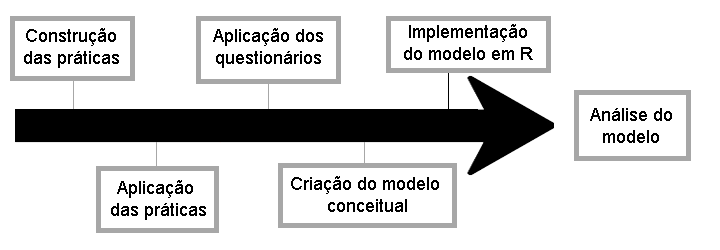
\includegraphics[width=14cm,height=4cm]{Imagens/Procedimento.png}
    \caption{Procedimentos}
    \label{fig:Procedimento}
\end{figure}

Nesta subseção encontram-se as descrições dos artefatos a serem utilizados no experimento e das etapas a serem cumpridas. A realização do experimento ocorre por meio da aplicação de questionários (online via \textit{Google Forms}) -- cujos detalhes são debatidos a seguir --, a fim de colher \textit{feedbacks} sobre a satisfação dos alunos com o processo de aprendizagem e sobre a percepção do professor do desempenho da turma \cite{chatley2017lean}. As perguntas são focadas em medir o quanto as atividades práticas nas disciplinas sobre as quais o experimento é executado estão agregando à formação dos alunos, em termos de fixação de conhecimento e conformidade com as demandas do mercado de trabalho \cite{chatley2017lean}. Busca-se tentar compreender se existe a percepção de que determinadas atividades e conhecimentos não são úteis ou são menos relevantes em detrimento de outros.

A decisão de criar questionários para obter os resultados do trabalho partiu de dois trabalhos, sendo eles o de Bandeira (2003)\nocite{Questionarios1} e de Henkel (2017)\nocite{Questionarios2}. Em ambos são apresentados métodos para análise de respostas abertas e fechadas em questionários. Para os resultados deste trabalho, utiliza-se parte dos métodos descritos por ambos, onde é necessário interpretar a fundo as respostas abertas e explorar as métricas obtidas com as respostas fechadas.

%Para o experimento espera-se conseguir o auxílio de dois professores especialistas do curso da Engenharia de \textit{Software}, dispostos a ajudar na experimentação da metodologia \textit{Lean Learning} durante um período letivo em sua disciplina. Com isto, espera-se que aproximadamente sessenta alunos participem do experimento. A escolha do especialista foi baseada em: i) seu conhecimento prévio sobre \textit{Lean}; ii) relação da sua disciplina com a metodologia; iii) período que a disciplina está alocada no curso. Busca-se abranger alunos iniciados e experientes, possibilitando uma amostragem diversificada de alunos e especialistas.
Para o experimento, conta-se com o auxílio da professora -- conhecida como especialista, conforme os atores especificados pelo processo do \textit{Lean Learning} -- do curso de Engenharia de \textit{Software} da PUC Minas, que lecionará a disciplina de Gestão da Produção de \textit{Software} no primeiro semestre de 2021. Ela foi contatada pelos autores e concordou em ajudar na experimentação da metodologia durante um período letivo em sua disciplina. Como espera-se atingir uma massa de pelo menos 60 respostas, outros professores foram contatados para contribuição no experimento. A escolha do professor (especialista) é baseada em: i) relação da sua disciplina com metodologias ágeis, processos de software e gestão \textit{Lean} e ii) período em que a disciplina está alocada no curso. 

Como há a possibilidade de as disciplinas selecionadas para o trabalho sofrerem conflito (concorrência) de horários e pelo menos um dos dois pesquisadores deve acompanhar a execução das práticas em cada disciplina no decorrer do semestre, eles podem ter que se dividir na execução destas. Essa divisão compreende também a aplicação dos questionários.

Busca-se trabalhar com alunos que estejam matriculados em disciplinas do segundo período em diante, pois supõe-se que normalmente é a partir desse momento que estão começando a adentrar o mercado de trabalho (ou estão próximos disso). Essa suposição é feita com base nos conhecimentos adquiridos até o terceiro período, pois nesta fração do curso os alunos já aprenderam alguns conteúdos basilares da Engenharia de \textit{Software}, como Algoritmos e Estruturas de Dados e Programação Modular, por exemplo -- e com esses conhecimentos, já estão minimamente aptos a ingressar no mercado de trabalho, ocupando cargos de entrada. Também é suposto que esses alunos sejam capazes de analisar por conta própria os benefícios do aprendizado na academia em seu dia a dia profissional, visto que já trabalham na área.

\subsubsection{Descrição das atividades práticas}

Neste trabalho espera-se estudar a etapa de Medir. Para isso, foram propostas atividades práticas -- em conjunto com a professora de Gestão da Produção de \textit{Software} -- que serão acompanhadas pelos autores deste trabalho e servirão como os protótipos no desenho do processo. Essas atividades são: 

    \begin{enumerate}\setlength\itemsep{0.5em}
        \item Prática envolvendo compreensão e refinamento de requisitos de software.
        \item Prática envolvendo trabalho em equipe, velocidade e competitividade.
        \item Prática envolvendo trabalho em equipe, brainstorming, criatividade e comunicação.
    \end{enumerate}

Na prática 1 propõe-se que os alunos se organizem em trios. Um dos alunos deve elaborar requisitos para uma tela de um sistema de sua escolha. Apenas através de texto, os requisitos da tela devem ser descritos e passados para os outros dois alunos. Ao receberem os requisitos, os dois devem ilustrar uma tela (na ferramenta de sua escolha) de acordo com as especificações dadas, de forma individual. Ao final da elaboração das telas, haverá uma reflexão com os alunos mediada pelo professor, sobre o que se esperava na tela e porque a tela foi feita daquela maneira. Espera-se que seja possível analisar pontos da etapa da elicitação de requisitos, como a fragilidade de requisitos ambíguos ou mal descritos e também como a interpretação dos requisitos pode alterar o resultado. Estima-se que essa atividade prática demande 30 minutos.

Na prática 2 uma lista contendo 4 problemas de programação serão apresentados aos alunos, que devem se organizar em grupos de 3 ou 4 integrantes. Durante 30 minutos eles devem resolver o máximo de problemas que conseguirem, podendo se organizar como quiserem -- decidindo como será a divisão de tarefas entre os membros, quais linguagens, recursos e ferramentas serão utilizados etc. Essa prática possui quatro restrições: 
    \begin{enumerate}\setlength\itemsep{0.5em}
        \item Os alunos terão apenas 30 minutos para a resolução dos problemas;
        \item Todos os integrantes dos grupos devem atuar na resolução dos problemas (ou seja, nenhum deve ficar ocioso);
        \item Todos os grupos formados devem operar de forma individual, não podendo haver cooperação entre eles;
        \item Ao final do tempo dedicado à resolução dos problemas, os alunos devem entregar um arquivo compactado (.zip, .rar ou .tar) contendo todas as soluções, de modo a garantir que nenhum código se altere após o prazo.
    \end{enumerate}
Para avaliar a resolução dos problemas, serão verificados apenas os conjuntos de saídas para cada conjunto de entradas testado, desconsiderando a implementação adotada no código. Essa atividade visa estimular trabalho em equipe, agilidade, coordenação e uma competição saudável entre os alunos. De modo a estimular a competição, será negociada a possibilidade de dar pontos extras (até 2) como prêmio aos membros da equipe vencedora, em cada disciplina em que a prática for aplicada. Essa atividade prática demanda 30 minutos. Os problemas de programação encontram-se no apêndice deste trabalho. 

 Na prática 3, os alunos de toda a turma serão considerados um grupo, será apresentado um vídeo com o título ``Os problemas da educação atual.", do canal ``Projeto EducatuX" e este será a base principal da prática. Os alunos devem chegar a um consenso sobre qual é o problema principal abordado no vídeo e propor uma solução em modelo de software para tal problema. Também será requisitado que citem e expliquem 4 requisitos funcionais e 2 requisitos não funcionais do modelo proposto pelos mesmos. Essa prática visa exercitar o trabalho em equipe e a comunicação com um grande número de pessoas, além de estimular a criatividade para solução de problemas. A prática tem como tempo limite 30 minutos de duração. Nessa prática devem ser gerados os seguintes artefatos:
\begin{itemize}\setlength\itemsep{0.5em}
    \item Uma descrição do problema abordado no vídeo.
    \item Uma descrição de um software que auxilie na solução do problema.
    \item Lista de requisitos do software descrito anteriormente.
\end{itemize}
Todos os artefatos devem ser postados em um formulário do \textit{Google} e então os pesquisadores podem analisar as ideias propostas. Essa prática possui várias soluções possíveis e não há competição, visto que todos os alunos serão do mesmo grupo e terão o mesmo objetivo\nocite{VideoPrat3}.

Espera-se que os demais professores que aceitem participar do experimento concordem em aplicar essas práticas dentro do contexto de suas disciplinas. Para manter a consistência dos resultados, busca-se aplicar as práticas e o experimento proposto em disciplinas que estão ligadas aos temas das práticas, como Engenharia de Requisitos, Arquitetura de Software, Medição e Experimentação em Engenharia de Software e afins. 

A etapa Medir utiliza das atividades práticas para gerar os dados que são analisados e servem como \textit{feedback} para o professor e também como a fonte de informações desse trabalho. Pretende-se medir métricas como: i) satisfação dos alunos com as atividades práticas; ii) satisfação do professor com o engajamento e desempenho da turma; iii) relação das atividades práticas com o mercado de trabalho.

\subsubsection{Questionários fechados}
%questionário fechado alunos

%Na primeira etapa do trabalho, será necessário desenvolver um questionário fechado (de múltipla escolha) destinado aos alunos, contendo questões que abordem: i) satisfação com as notas obtidas; ii) satisfação com o aprendizado; iii) participação nas aulas; iv) participação nas atividades práticas; v) aprendizado com atividades práticas; vi) proximidade entre conteúdo aprendido e demandas do mercado. Cada item descrito será avaliado com notas de 1 a 5, onde o valor 1 representa insatisfação, e o valor 5 representa muita satisfação com os resultados.
Na primeira etapa do trabalho, utiliza-se o questionário fechado (de múltipla escolha) destinado aos alunos, contendo questões que abordem: i) satisfação com o aprendizado proporcionado pela atividade prática; ii) participação nas atividades práticas; iii) dificuldade para fazer a prática; iv) proximidade entre a atividade e práticas e demandas do mercado. Cada item descrito é avaliado com notas de 1 a 5, onde o valor 1 representa insatisfação, e o valor 5 representa muita satisfação com os resultados.

%questionário fechado profs
Também é utilizado um questionário fechado destinado aos especialistas. Este questionário tem questões considerando percepções de: i) engajamento dos alunos em relação a atividade prática; ii) complexidade da prática realizada; iii) desempenho dos alunos na atividade proposta; iv) fixação do conhecimento pela atividade; v) proximidade entre a prática e demandas do mercado. As respostas também vão variar entre 1 e 5, onde o valor 1 representa insatisfação, e o valor 5 representa muita satisfação com os resultados.

Com ambos os questionários fechados pretende-se realizar uma análise da média móvel e regressão linear com os dados coletados baseados nas respostas dos participantes. As medidas encontradas são utilizadas para definir a conclusão do artigo sobre a viabilidade do uso do \textit{Lean Learning} no ensino da Engenharia de \textit{Software}.
%quando aplicar
%Ambos os questionários citados são aplicados de 15 em 15 dias a fim de manter um \textit{feedback} constante tanto dos alunos quanto dos professores em relação a metodologia, podendo assim analisar rapidamente práticas que possam ser prejudiciais e mapear possíveis correções. A finalidade dos questionários fechados é permitir a obtenção de \textit{feedbacks} estruturados em termos quantitativos, de modo que seja possível estabelecer métricas para medir a satisfação dos alunos com seu aprendizado nas disciplinas.  %A conclusão de que esse seria o caminho mais viável a ser tomado para a medição qualitativa deu-se a partir do fato de que não seria factível agendar entrevistas individuais com todos os alunos, mas com os professores seria, dadas as proporções numéricas da pesquisa.
\subsubsection{Questionário aberto}
%aberto e entrevista
O questionário aberto visa a obtenção de: i) percepções dos alunos não contempladas no questionário fechado; ii) manifestação livre de suas opiniões acerca do aprendizado e das práticas; iii) \textit{feedbacks} de possíveis melhorias nas disciplinas. Para observar a satisfação de forma qualitativa, analisa-se as respostas do questionário aberto, a ser aplicado aos alunos. Tais respostas precisam ser interpretadas e simplificadas a tópicos principais discutidos nelas, para então se realizar uma análise de tópicos. O propósito destes é permitir colher respostas livres dos participantes, de modo que possam expressar suas opiniões sobre o processo de aprendizagem a partir de suas próprias perspectivas. Os questionários são realizados em três momentos diferentes, como visto nas Tabelas 1 e 2, as mesmas ocorrendo logo após cada prática aplicada aos participantes. 

%Ao final do experimento, espera-se que seja possível observar os pontos positivos comuns entre os diversos especialistas que auxiliaram, e assim indicar fatores que despertam o interesse dos alunos com relação ao ensino da Engenharia de \textit{Software}. Além disso, também é possível analisar a relação da disciplina com o mercado de trabalho e de forma constante buscar uma evolução ainda maior no método de ensino. %Tendo em vista a participação de seres humanos neste estudo, caso o projeto seja aprovado, ele será submetido ao Comitê de Ética em Pesquisa da PUC Minas para análise, de acordo com instruções disponibilizadas pela universidade (https://www.pucminas.br/pesquisa/Paginas/comite-de-etica-em-pesquisa.aspx).